




%\begin{figure}[!h]
%\centering 
%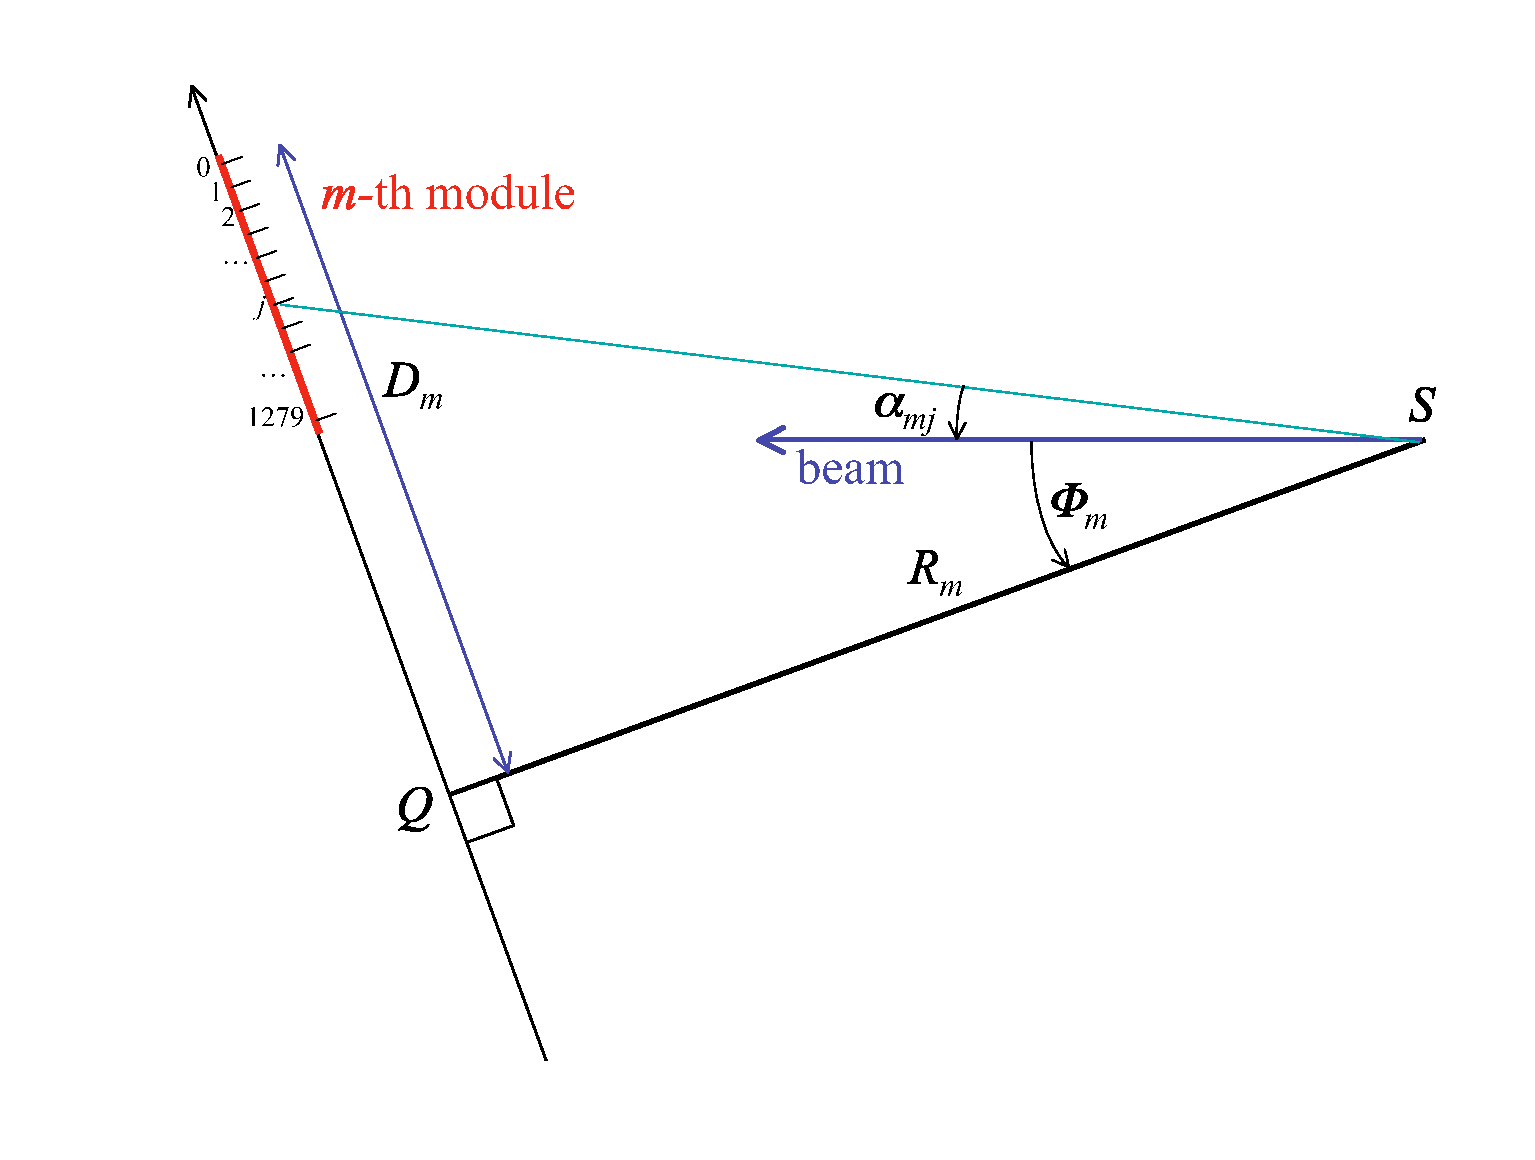
\includegraphics[width=0.98\textwidth]{AngConv}
%\caption{Schematics of the scattering geometry in the diffraction plane. A Mythen II module is shown. $R_m$ is the distance from the module sensor plane (orthogonal to the diffraction plane) to the sample position $S$; $D_m$ the distance from the center of pixel $j=0$ to point $Q$, counted positively as the arrow on the module plane goes (\emph{i.e.}, oppositely to the direction of increasing $j$); $\Phi_m$ is the angle of the module plane normal with the beam direction, positive counterclockwise. $\alpha_{jm}$ is the angular position of the $j$-th pixel center with respect to the beam direction, positive counterclockwise.}
%\label{acon}
%\end{figure}

Mythen II modules are composed by 1280 pixels, each having width p=0.05~mm, and numbered with j=0,..,1279. 
Angles are counted counterclockwise from the beam direction. For the m-th module, the angle $\alpha_{jm}$ of its j-th pixel center 
can be determined using the three geometric parameters $R_m$~[mm], $\Phi_m$~[deg], $D_m$~[mm], as in \fref{acon}. 
The detector group uses instead the 3 parameters center $c_m$~[\ ], offset $o_m$~[deg], conversion $k_m$~[\ ]. 
The law with the 3 geometric parameter is
\begin{equation}
\alpha_{jm}=\Phi_m-\lrb{\DSF{180}{\pi}}\arctan\lrb{\DSF{D_m-pj}{R_m}}
\end{equation}
The corresponding law using DG's parameters is
\begin{equation}
\alpha_{jm}=o_m+\lrb{\DSF{180}{\pi}}c_mk_m+\lrb{\DSF{180}{\pi}}\arctan\lrs{\lrb{j-c_m}k_m}
\end{equation}
One can convert the two forms by equating separately the term out of the arctan and the argument of arctan for two different values of j. 
It results
\begin{eqnarray}
c_m&=&\DSF{D_m}{p};\\ 
k_m&=&\DSF{p}{R_m};\\ 
o_m&=&\Phi_m-\DSF{180}{\pi}\DSF{D_m}{R_m}.
\end{eqnarray}
Conversely,
\begin{eqnarray}
\Phi_m&=&o_m+\DSF{180}{\pi}c_mk_m;\\
R_m&=&\DSF{p}{k_m};\\
D_m&=&c_m p.
\end{eqnarray}
